\chapter{Experiments}
\label{chapter:experiments}

In this chapter, we will look at the the configuration of experiments that has a direct impact on the results of our four different anomaly detection approaches. Before conducting the experiments, we will also look at the data visually to check the correctness of assumptions we hold about the data. After that, we will introduce the experiment setup including datasets, software and hardware used for experiments and evaluation matrics. Finally, we present the definitions of tunable hyperparameters and provide an overview of the hyperparameter values that performed best and are used for final experiments.

\section{Exploration of Assumptions}
To get a better insight into the dataset, it is useful to perform an initial Exploratory Data Analysis (EDA) \cite{eda} of our dataset. Exploratory data analysis is being used to analyze the underlying structure of the data and summarize the main characteristics, often via visualization methods. The visualization helps us to check our assumptions and formulate hypotheses of the data, which are important to choose the correct anomaly detection approaches and parameters. In addition, being able visualize the logs will help us answer \textbf{RQ1} (Research Question 1).

For visualization, we use the numerical representation of our dataset that we obtained by feature extraction. All the visualizations in the sections below were obtained on the event count embedding of the data. The embedding of log sequences contains \featureVectorLength\ variables. Data of such high dimensions are difficult to interpret. Therefore, it is necessary to use dimensionality reduction techniques. To perform an initial exploration as well as to visualize the results of anomaly detection, we will employ two algorithms, PCA and t-SNE, to reduce the dimensionality for data visualization:

\begin{itemize}
    \item \textbf{Principal Component Analysis (PCA)} \\
    One way of reducing the dimensionality of data without losing too much information is to use Principal Component Analysis (PCA) as an unsupervised tool for exploratory data analysis. 
    In PCA, the data points (in our case, feature vectors) in our\\ \featureVectorLength-dimensional feature space are transformed onto a 2-dimensional feature subspace. Furthermore, the variables in the new artificial subspace (principal components) are not correlated. The first principal component (PC1) spreads in the direction of the x-axis and explains the most variance in the data.
    
    \item \textbf{t-distributed Stochastic Neighbor Embedding (t-SNE)}\\
    t-SNE is a more recent algorithm for dimensionality reduction into a space of two or three dimensions, that is particularly well-suited for data visualization \cite{tsne}. PCA is a linear technique that keeps the dissimilar datapoints in the low-dimensional projection far apart. In contrast with PCA, t-SNE is a non-linear technique. It focuses on retaining the local structure by keeping the high dimensional datapoints that lie on or near a non-linear manifold in lower dimensions close together. Retaining local structure, while also revealing an important global structure, is the biggest advantage over linear techniques, where this is usually not possible.
    
\end{itemize}

The four assumption that we are going to explore regarding the collected data are the following: 

\begin{itemize}
    \item \textbf{Assumption 1:} Daily dataset varies too significantly from normal behaviour represented by Nightly to be used for training
    \item \textbf{Assumption 2:} Using data from nightly testing collected from a single night for training is sufficient, as data from every nightly testing are equivalent
    \item \textbf{Assumption 3:} Logs produced during calls between two radios are grouped in a cluster of calls when plotted
    \item \textbf{Assumption 4:} Different anomaly logs are grouped into distinct and clearly separated clusters when plotted
\end{itemize}

We will describe each assumption in detail in the next sections.

\subsection{Choosing Data for Training: Daily vs Nightly}]
\label{assumption-daily-vs-nightly}

As we explained in the earlier sections of this chapter, we train the models on the Nightly dataset under the assumption that its data points are normal. On the other hand, we have no prior assumptions about the Daily dataset and about the distributions in it. Thus, we want to perform a simple visual comparison of the Daily and Nightly dataset. Next, we sought to determine whether the data points from the day fall within the normal region.

In Figure \ref{fig:tsne-single}, there are two visualizations of applying t-SNE to the the Nightly and Daily datasets correspondingly. t-SNE analysis of the Daily data appears to separate the data into four visual clusters. While it is difficult to interpret what each of the clusters represents even for domain experts, we suppose that at the day of obtaining the Daily dataset, the developers were testing out four different features \todo{restructure}, and that as a consequence led to the groupings of data points into clusters.

The visualization of the t-SNE in the plot of the Nightly dataset shows that most of the data points are packed together and form a cluster. However, there is a cluster of points at the bottom of the plot, that appears to be fairly distant from the rest of the points and might be considered to be a set of outliers. Upon closer inspection of the raw logs behind the data in this cluster, we discovered that they contain a high number (around $400$ hundred logs every two minutes) of log messages informing a call was happening, as illustrated by the following event templates:

\begin{itemize}
    \item \texttt{\justify Call \{1586,1\} \{:call\_number, <*> <*> forwarding audio RtpPacket\{ssrc: <*> urid: <*> timestamp: <*> seq\_num: <*>}
    \item \texttt{\justify Call \{1586,1\} \{:call\_number, <*> <*> received RtpPacket\{ssrc: <*> urid: <*> timestamp: <*> seq\_num: <*> from \{228, 28, <*> <*>}
    \item \texttt{\justify Call \{1586,1\} \{:call\_number, <*> <*> forward RtpPacket\{ssrc: <*> urid: <*> timestamp: <*> seq\_num: <*> LMR: [ssrc: <*> urid: <*> to \{228, 28, <*> <*>}
\end{itemize}

This is further confirmed by visualizing the Call dataset in respect to the Nightly dataset in Assumption \ref{assumption-calls}.

As calls are not happening frequently during the testing phase, comparing to other processes that are happening in the system, this is precisely what we expect to be reflected in the logs. Nevertheless, as shown in the plot, the cluster is considerably distant from the rest of the points and we do not want regular calls to be detected as anomalies. Here it is important to note that the distances between clusters in t-SNE do not necessarily have to mean something. To obtain clusters that retain global geometry, it is required to fine-tune the \textit{perplexity} hyperparameter of t-SNE. Thus, we do not know where does the assumed call cluster lies with respect to the rest of the data points.

\begin{figure}%
    \centering
    \subfloat[\centering Nightly Dataset]{{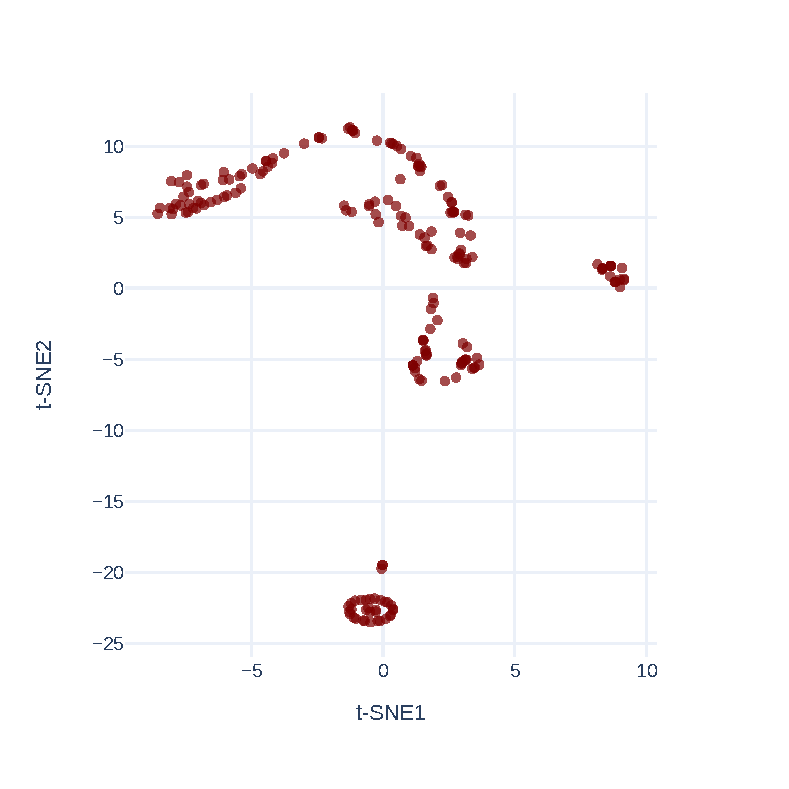
\includegraphics[width=5.52cm]{img/tsne-nightly.pdf} }}%
    \qquad
    \subfloat[\centering Daily Dataset]{{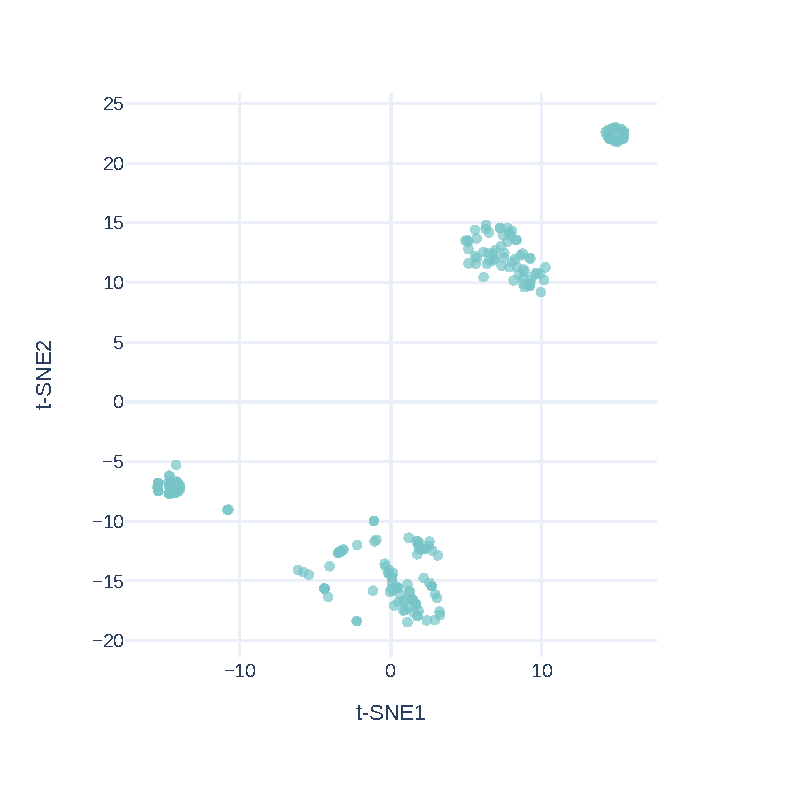
\includegraphics[width=5.52cm]{img/tsne-daily.pdf} }}%
    \caption{Application of t-SNE on the event count vector embeddings of the Nightly and Daily datasets.}%
    \label{fig:tsne-single}%
\end{figure}

Finally, we are interested to see how does the PCA perform in comparison to t-SNE and we also want to plot both Daily and Nightly dataset with respect to each other. Figure \ref{fig:pca-nightly-daily} displays a plot of the first two principal components after performing principal component analysis on the Nightly and Daily dataset. Figure \ref{fig:tsne-nightly-daily} is a t-SNE plot visualizing the Nightly and Daily datasets.

The points produced by PCA appear to be much more crowded in comparison with t-SNE, however in both plots there is a very little intersection between Daily and Nightly data. One way to explain this is that the tests performed during the night do not completely cover the behaviour of the system. Another explanation, that was confirmed by the developers at Motorola as the most likely, is that the experiments performed during the day vary each day depending on the feature that is being tested and it may also behave completely counter to what we consider a normal behaviour. Nevertheless, these visualizations confirmed, that the Daily dataset should not be used for training the models as it's unpredictable and inconsistent. It is still a good candidate for performing expert validation on unlabeled dataset, where an expert's understanding of underlying processes will help us understand the anomaly detection models.

\begin{figure}[h]
    \centering
    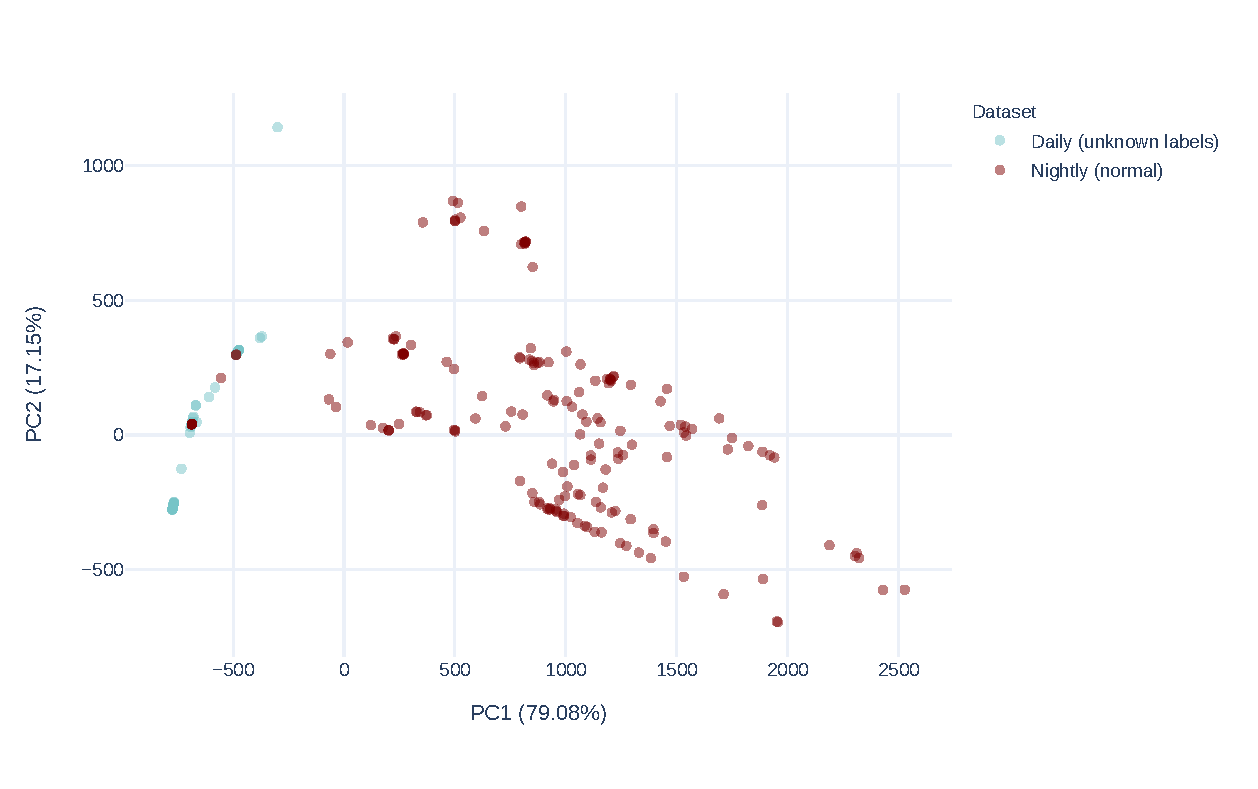
\includegraphics[width=\textwidth]{img/pca-nightly-daily.pdf}
    \caption{Application of PCA to the Daily and Nightly dataset}
    \label{fig:pca-nightly-daily}
\end{figure}

\begin{figure}[h]
    \centering
    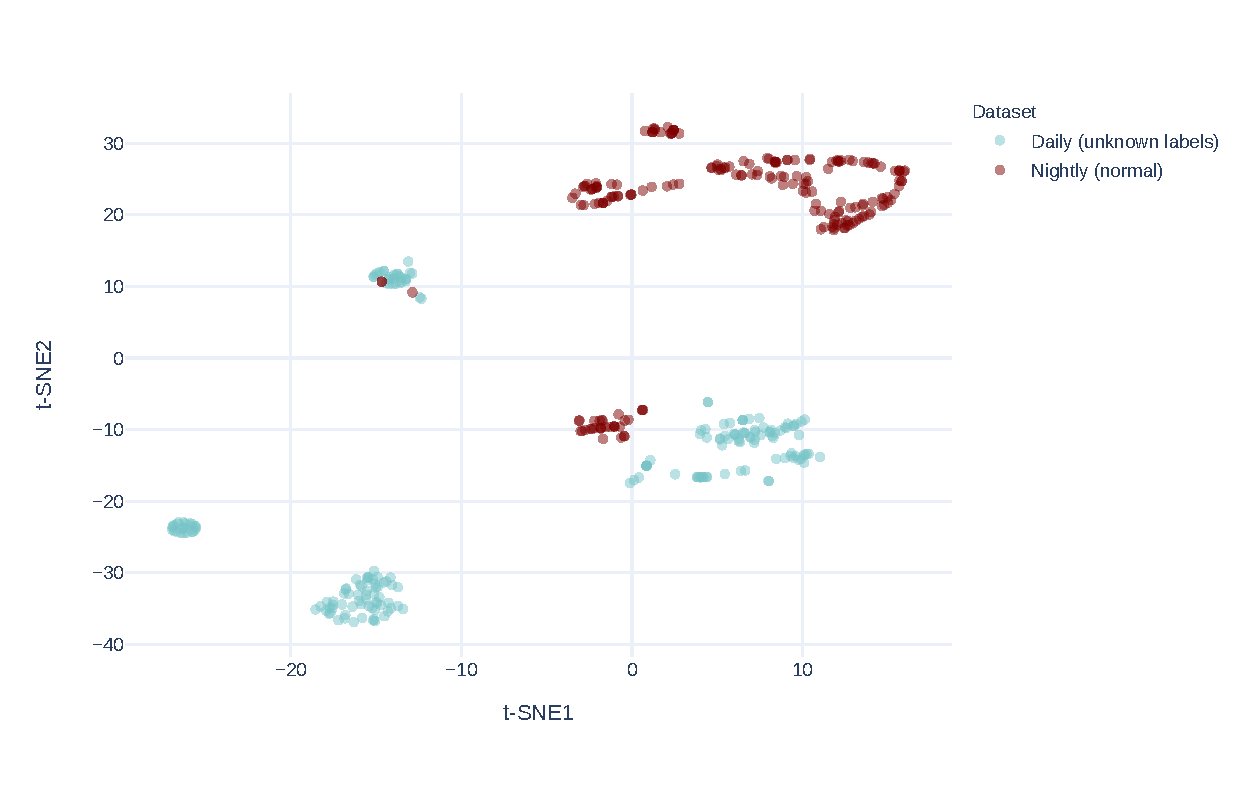
\includegraphics[width=\textwidth]{img/tsne-nightly-daily.pdf}
    \caption{Application of t-SNE to the Daily and Nightly dataset}
    \label{fig:tsne-nightly-daily}
\end{figure}

\subsection{Completeness of the Nightly Dataset}
\label{assumption-completeness}

Another set of important questions we would like to answer by conducting EDA are concerning the completeness of Nightly dataset obtained on 24 January, 2021, that we plan to use for one-class model training: \textit{Do data from nightly testing differ among different dates?} \textit{Would merging data from several nightly testing datasets provide some extra information about the normal behaviour of the system?}

To analyze the data and answer these questions, we will again use PCA and t-SNE and plot data obtained during two different nights of testing. Figure \ref{fig:tsne-nights-comparison} gives the visualization of the results. We can observe that the two datasets overlap almost entirely in both PCA and t-SNE plots. From the substantial overlap we can safely assume that logs gathered during the nightly testing are equivalent within the different dates.

By our domain knowledge, we know that the code under the tests is going to slightly differ, as the software product of Motorola SmartConnect is being developed. The reason is that master branches of services are being tested and we do not expect them to be changing dramatically day to day. 
However, it is something that has to be taken into account when deploying our solution. It has to be verified that the code whose produced logs are being analyzed by our anomaly detection algorithm is also the version of code that runs the tests.

We conclude that using data from just one night is enough for training the anomaly detection models and adding more logs from different nights would not bring any extra information to the data. 

\begin{figure}%
    \centering
    \subfloat[\centering PCA]{{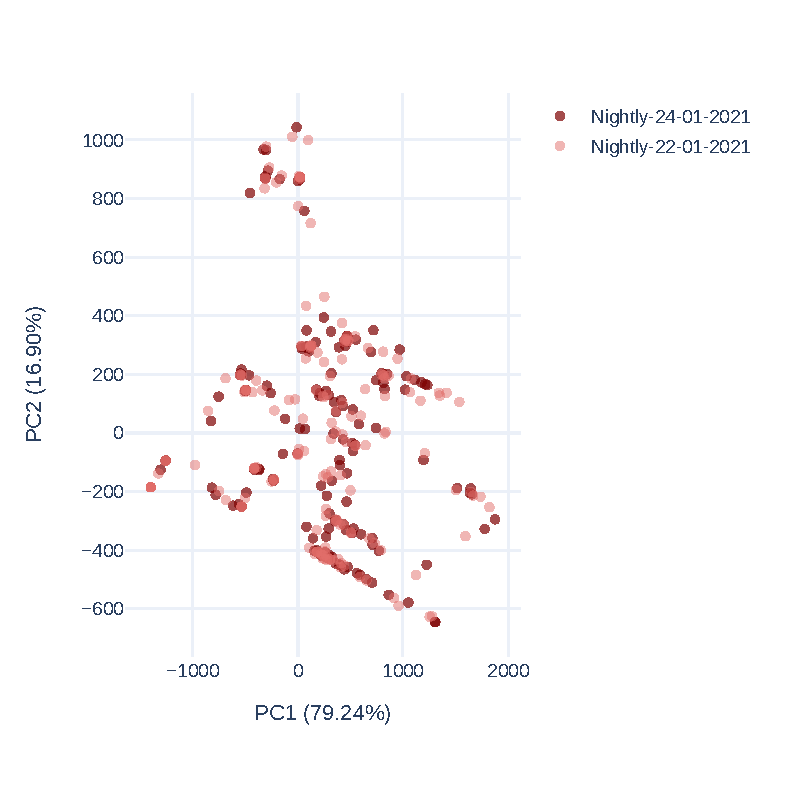
\includegraphics[width=5.52cm]{img/pca-nights-comparison.pdf} }}%
    \qquad
    \subfloat[\centering t-SNE]{{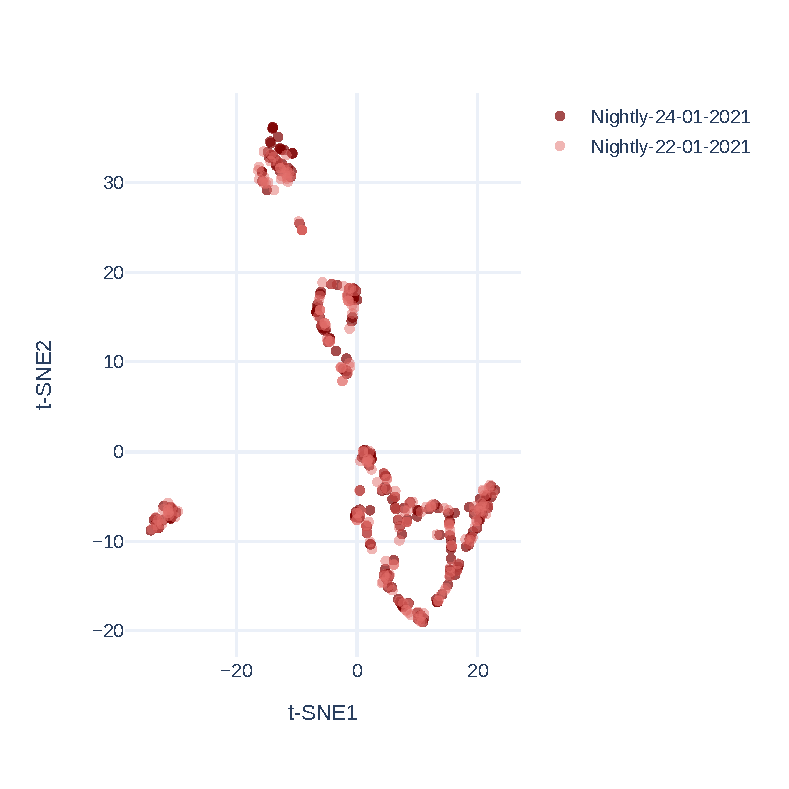
\includegraphics[width=5.52cm]{img/tsne-nights-comparison.pdf} }}%
    \caption{Comparing data from nightly testing obtained from two different dates.}%
    \label{fig:tsne-nights-comparison}%
\end{figure}


\subsection{Calls Group Into A Cluster}
\label{assumption-calls}
In the t-SNE of the Nightly dataset, we could see a cluster of points that we assumed are calls being made between two radios. The assumptions stems from us choosing several random data points (log sequences) from that cluster and hand-checking the histogram of log templates within the log sequences. It appeared that a vast majority of them represented calls. We want to prove that the observed point grouping is a cluster of call logs and it is not an unknown anomaly. We will prove this assumption by highlighting the Glostrup Calling dataset created specifically for this purpose in the t-SNE embedding of the Nightly dataset as a central point of reference about where do the call data points cluster.

Figure \ref{fig:tsne-nightly-calls} is depicting running t-SNE on the above described scenario. After applying feature extraction into $2$ minute windows on the simulated $8$ minutes of calls, we obtain $4$ data points (highlighted by green color). The visualization of the plot indicates that the call data points fall very close to the observed cluster and in addition, all of the call data points are consistently tightly packed together. 

Therefore, we believe that it is possible to determine the class of a clustered group of data points even without leveraging the actual labels. It confirms our assumption that the data from the Nightly dataset are anomaly free and that the observed cluster is indeed a cluster of calls.

\begin{figure}[h]
    \centering
    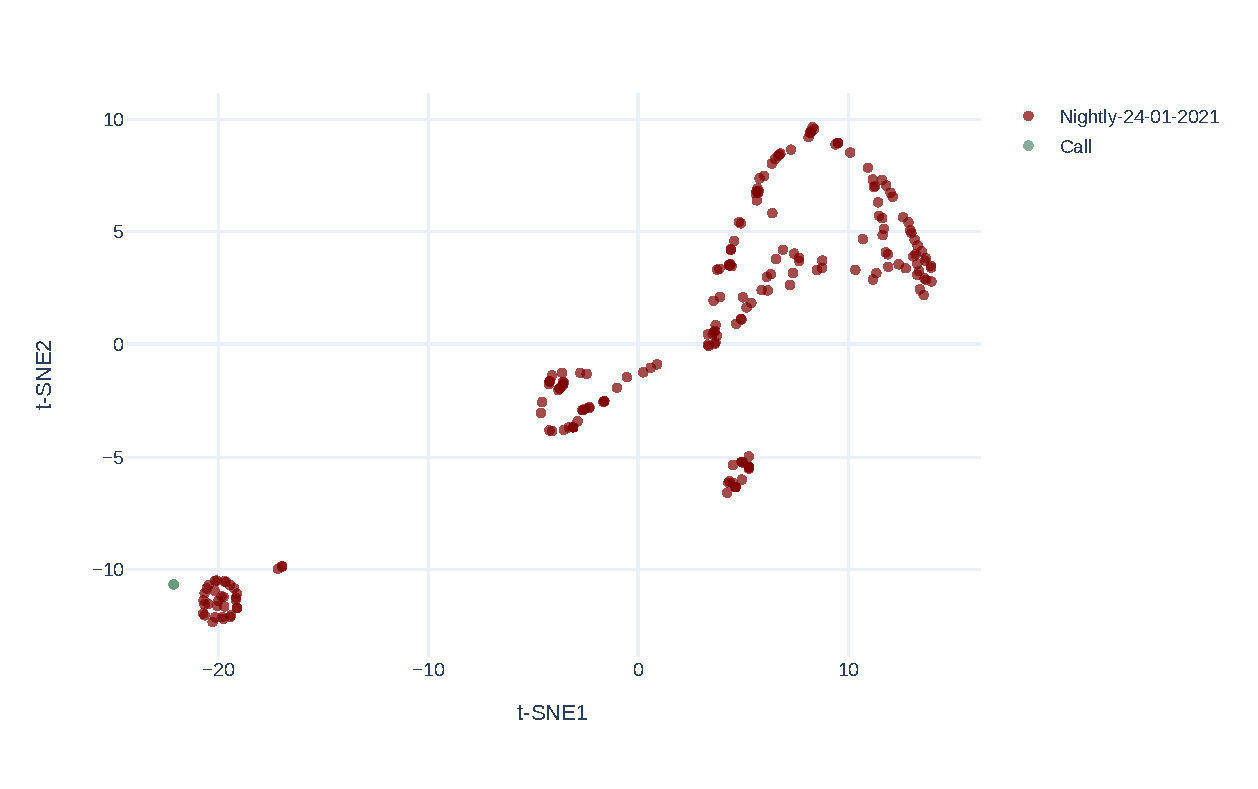
\includegraphics[width=\textwidth]{img/tsne-nights-call-comparison.pdf}
    \caption{Application of t-SNE to the Nightly and Glostrup Calling dataset.}
    \label{fig:tsne-nightly-calls}
\end{figure}

\subsection{Anomalies Are Separable from Normal Data}
\label{assumption-anomalies}
The last assumption which we want to verify before using the data to train actual machine learning models and considerably the most important one, is to look whether anomalies have a tendency to cluster together in different regions than normal data. It is crucial, because if human eye can detect an anomaly by looking at a plot, then we can assume that anomaly detection algorithms are also able to detect these anomalies. 

In order to prove that, we will plot our Anomalies dataset generated by collecting anomalies during simulation of anomaly scenarios described in Section \ref{anomaly_types}. In both PCA and t-SNE plots in Figure \ref{fig:pca-anomalies} and \ref{fig:tsne-anomalies} respectively, anomaly of killing the Redis is represented by green and killing the RabbitMQ is represented by blue color. Anomalous data points are plotted in respect to normal points, which are highlighted as red. 

Both plots give us a clear picture that the data points are split into distinct clouds of the same anomaly types. Moreover, the anomalous points are located outside of the normal region. We consider the fact that different anomalies can be successfully distinguished as clusters in the embedding space as an answer to the \textbf{RQ1}. In this case, it is clear that t-SNE gives us better clustering result than PCA with less point overlapping each other, even though both techniques are able to separate the data points into different classes. However, it is interesting to see in the PCA plot, that the Killing Redis anomaly is located much closer to the cluster of normal points than Killing RabbitMQ (as mentioned earlier, we should not take the distances between clusters in t-SNE plots into account unless tuning its parameters, that's why we focus on the PCA graph for cluster proximity analysis). This can be explained as an outage of all brokers in the distributed architecture of the system that relies on passing messages between microservices, which causes a major distortion of the whole infrastructure. 
While non-functioning Redis cache is an issue that can be overcome relatively easily, the latter one causes severe problem in the application, propagating to many places. Also, as we observed, the broken broker scenario makes the system disfunctional for a much longer time period giving services longer window for generating greater amount of logs indicating problems.

We got a solid indication that the feature embedding is informative enough to identify anomaly clusters. We will attempt to further prove this assumption by using machine learning.

\begin{figure}[!h]
    \centering
    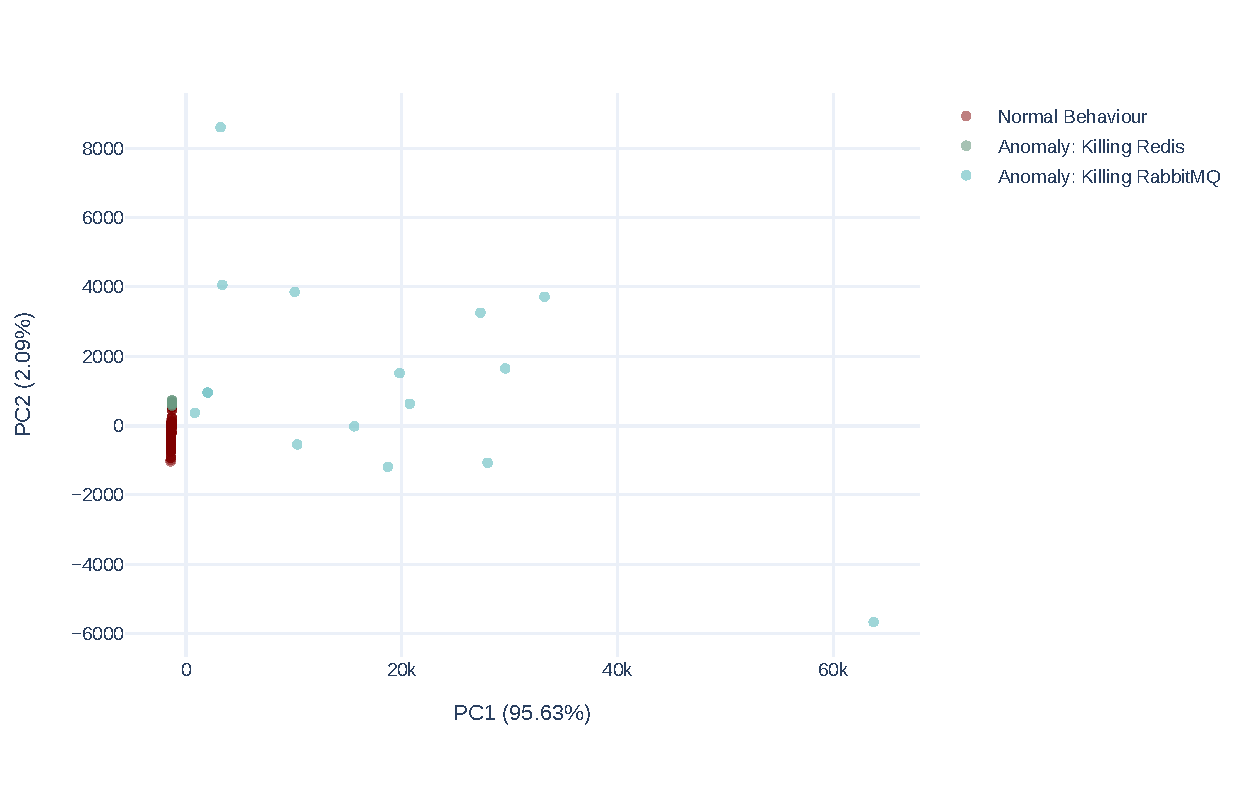
\includegraphics[width=\textwidth]{img/pca-anomalies-vs-normal.pdf}
    \caption{Application of PCA to the anomaly data.}
    \label{fig:pca-anomalies}
\end{figure}

\begin{figure}[!h]
    \centering
    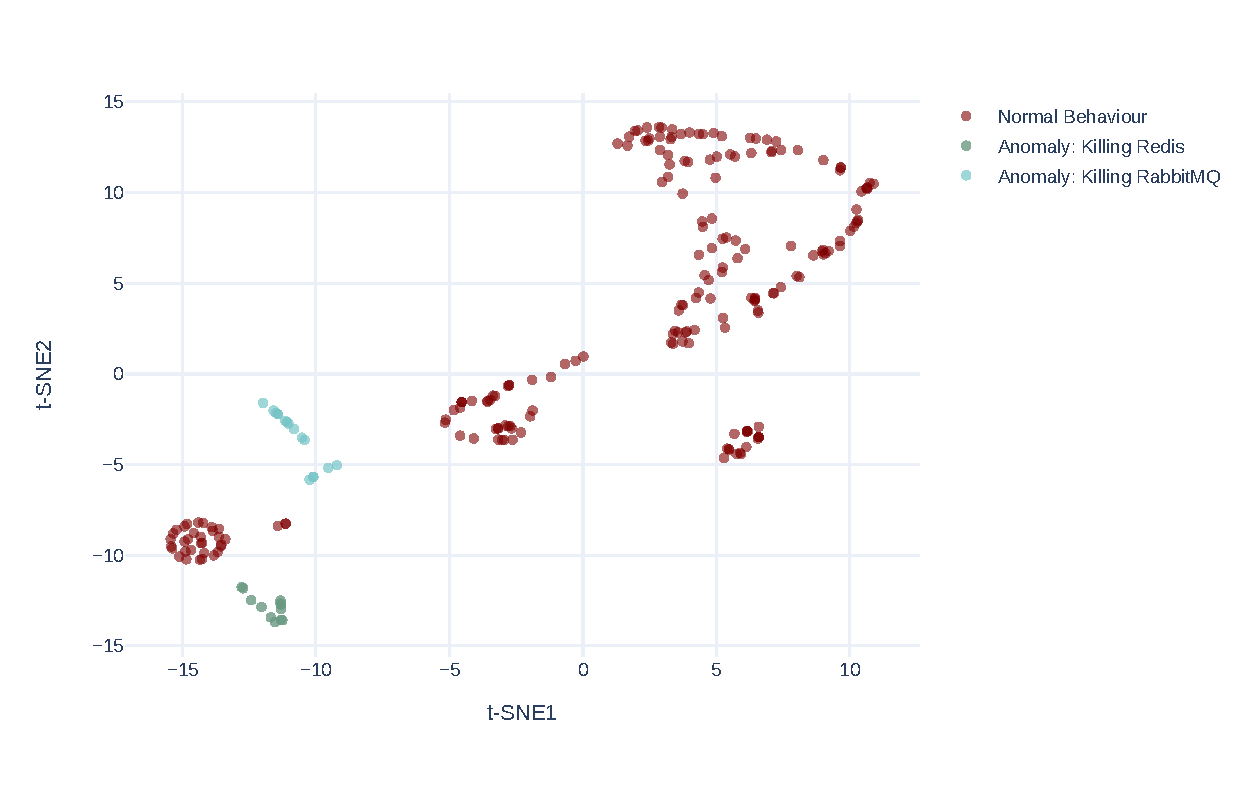
\includegraphics[width=\textwidth]{img/tsne-anomalies-vs-normal.pdf}
    \caption{Application of t-SNE to the anomaly data.}
    \label{fig:tsne-anomalies}
\end{figure}

\section{Evaluation Metrics}
\label{section:evaluationMetrics}
In order to appropriately compare different anomaly detection algorithms and different experiment settings, evaluation metrics are required.

Firstly, let's introduce four basic metrics: true positive (TP), false positive (FP), true negative (TN) and false negative (FN). 

To give an example, let's consider an experimental setting: in a classification task, for each data example we have assigned a binary label $l$ with values in a set of classes. It is important to note that one class, that is usually positive, is of special interest, for which the evaluation measure is valid. It gives an information about the correctness of the example given the anomaly detection task. Moreover, an anomaly detector produces a prediction $\hat{l}$, assigning for each data example whether it classifies it as an anomaly or a normal data instance. The pair-wise relationship the four counts is explained by the confusion matrix in Table \ref{table:confusionMatrix}. Confusion matrix is a form of contingency table, that allows interpretation of classifier's performance on a labeled dataset. It is a $2 \times 2$ matrix (in case of having only two classes, but can be easily extended for multiple classes), where rows represents an actual value of a variable, while columns represent the predicted value of a variable.

\begin{table}[!h]
\centering
\begin{tabular}{cccc}
\multicolumn{1}{r}{}                 &                              & \textbf{Predicted}          &   $\hat{l}$                          \\ \cline{3-4} 
                                     & \multicolumn{1}{l|}{}        & \multicolumn{1}{l|}{Anomaly} & \multicolumn{1}{l|}{Normal} \\ \cline{2-4} 
                                      
\multicolumn{1}{l|}{\textbf{Actual}} & \multicolumn{1}{l|}{Anomaly}  & \multicolumn{1}{l|}{\textcolor{customBlue}{\textbf{TP}}}     & \multicolumn{1}{l|}{\textcolor{customRed}{\textbf{FN}}}      \\ \cline{2-4} 
\multicolumn{1}{c|}{\textit{l}}                & \multicolumn{1}{c|}{Normal} & \multicolumn{1}{l|}{\textcolor{customDarkRed}{\textbf{FP}}}     & \multicolumn{1}{l|}{\textcolor{customGreen}{\textbf{TN}}}     \\ \cline{2-4} 
\end{tabular}
\caption{An example of a confusion matrix for binary classification.}
\label{table:confusionMatrix}
\end{table}
 
Many meaningful measures can be extracted out of the confusion matrix. The evaluation measures are calculated on the positive class, which is assumed to represent the presence of an anomaly.

\textit{Accuracy} is the most general metrics to measure performance. It simply measures the fraction of correct predictions from all the available data points. The computation of accuracy in binary classification is done as shown in the following equation:

\begin{align}
    Accuracy = \dfrac{TP + TN}{TP + TN + FP + FN}
\end{align}

However, accuracy alone does not exactly reflect the real performance of a system designed to correctly detect anomalies. It does not differentiate between the number of correct predictions of different classes \cite{performanceEvaluation2006}. The reason why accuracy measure is not enough in the majority of ML applications will be explained in the remainder of this section. 

The most typically used metrics for estimating performance in machine learning are \textit{precision, recall} and ${F_{\beta}-measure}$. They measure the correct prediction of anomaly within different classes. In our research, we will also focus on these three  performance indicators.

In order to use them, the problem for which we want to estimate performance must be a classification problem. We assume our dataset represents a normal behaviour of the system, thus an anomaly detection problem can be translated into a one-class classification problem. 

Precision, recall and $F_{\beta}$-measure rely on the ratios of TP, FP, TN and FN counts. 

Precision represents the fraction of correctly detected anomalies from the total number of reported anomalies. Recall measures the fraction of correctly detected anomalies from the total number of anomalous data points in the dataset. Lastly, $F_{\beta}$-measure combines both of these measures into a single measure. $F_{\beta}$-measure represents the harmonic mean of precision and recall. If precision and recall are evenly balanced, then $\beta = 1$ and we call it F1-measure. If $\beta > 1$, the score is in favour of precision. On the other hand, it is in favour of recall if $\beta < 1$. 

Let's look at the mathematical formulas for calculating evaluation measures:

\begin{align}
    Precision &= \dfrac{TP}{TP + FP} \\
    Recall &= \dfrac{TP}{TP + FN} \\
    F_{\beta}-measure &= (\beta^2 + 1) \cdot \dfrac{Precision \times Recall }{\beta^2 \cdot Precision + Recall} 
\end{align}

The reason for $F_{\beta}$ score is that improving either precision or recall on their own is a trivial task, but the goal is to optimize both of them at the same time. Accuracy metrics is more useful when true positives and true negatives are more important. However, false positives and false negatives are considered to be crucial in most of the classification problems. Thus, in these cases, $F_{\beta}$ score happens to be a better evaluation metrics. False negatives and false positives are given more weight while not letting large numbers of true negatives to influence the score.

In addition, as anomalies occur much less frequently than normal data samples, we can easily achieve a high accuracy without catching anomalies. That's why we will not use accuracy metrics for evaluation in this thesis.

\section{Experimental Setup}
\label{section:experimental-setup}
In Chapter \ref{chapter:literatureReview}, we have described four anomaly detection algorithms: Isolation Forest (\ref{section:lrIsolationForest}), PCA (\ref{section:lrPCA}), Invariant Mining (\ref{section:lrInvariantMining}) and Log Clustering (\ref{section:lrLogClustering}). These algorithms will be used to carry out the unsupervised anomaly detection experiments. In this section, we will describe the data used in these experiments and discuss the choice of different parameters for each of the anomaly detection methods. To tune the parameters, we will use the evaluation metrics described in previous section.

\subsection{Dataset}
The dataset used for training models is the Nightly dataset with data instances of normal class, thus we also refer to this type of learning as one-class learning. Before training, in all of our experiments indistinguishably, we start by preprocessing data into numerical vector embeddings following the methods described in Chapter \ref{methodology}. In Table \ref{tab:training} we give an overview of the statistics regarding the dataset used for training and testing.

We used the sliding window technique to divide the dataset into log sequences. The number of resulting sequences depends on the size of the window and a size of the step.  The window size should be set such that it contains the maximal amount of information. We have identified that the anomalies we observe in the experiments spawn at most two minutes. Therefore, we set the window size to two minutes, and the step size into two minutes as well, so that no two windows overlap. As a result we got $201$ log sequences extracted out of the Nightly dataset. Each log sequence can be one of two different vector representations: \textit{event count} vectors and \textit{TF-IDF} weighted vectors. Thus, we will run each experiment twice on both embedding types.

The length of a vector is given by the number of unique event templates, that were extracted and stored in our log template miner's state during the preprocessing of all datasets used in our research. Thus, by the time of model training, the number of event types as well as the length of each log sequence is equal to $3\,963$.

% Please add the following required packages to your document preamble:
% \usepackage{booktabs}
% Please add the following required packages to your document preamble:
% \usepackage{booktabs}
\begin{table}[h]
\centering
\resizebox{\textwidth}{!}{\begin{tabular}{@{}ccccc@{}}
\toprule
\textbf{Dataset} & \textbf{Window size} & \textbf{\# Log sequences} & \textbf{\# Event types} & \textbf{Ratio of anomalies} \\ \midrule
Nightly          & 2 minutes            & 201                       & 3693                    & 0                           \\
Testing          & 2 minutes            & 131                       & 3693                    & 0.22                        \\ \bottomrule
\end{tabular}}
    \caption{Summary of statistics of the Nightly dataset used for training and Testing dataset used for model evaluation and hyperparameter tuning.}
    \label{tab:training}
\end{table}

\subsection{Software}
To develop data preprocessing scripts and to conduct our experiments, Python 3.6.9 was used as a primary programming language. In addition, we used the following Python libraries: 

\begin{itemize}
    \item pandas 1.1.3
    \item numpy 1.19.2
    \item torch 1.7.1
    \item plotly 4.12.0
    \item matplotlib 3.3.2
    \item jupyterlab 2.2.8
\end{itemize}

Exploratory analysis, data plotting and the preparations of scripts for the ML pipeline are performed using Jupyter Notebook with a Jupyter Lab interface for browsing files. Jupyter Notebook is a web-based interactive computational environment for writing python code, that operates in a web-based environment. The biggest advantage in using Jupyter Notebook instead of writing Python scripts directly is the ability to execute inline code and see the result directly beneath it. It also allows to add formatted texts that improves the readability and reasoning behind the analysis steps.

\subsection{Hardware}
All experiments were conducted on a HP ZBook machine with the following technical specification:
\begin{itemize}
    \item Operating System: Linux Mint 19.3 Cinnamon
    \item CPU: Intel Core i7-8850H
    \item RAM Size: 32 GB
    \item CPU Frequency: 2.60 GHz
    \item Internal Storage: 500 GB
\end{itemize}

\subsection{Algorithm Hyperparameters}
Hyperparameters are the values of parameters that are used to configure a machine learning model and they must be set before the learning process, which is the main difference between parameters, which are found \textit{during} the learning process. As the performance of the model on given combination of dataset and hyperparameters is not known, it is required to explore the range of possible values to obtain optimal hyperparameters. This optimization process is called \textit{tuning}.

The strategy we follow to find optimal parameters is a simple grid search: For each combination of hyperparameter values, we train a model and look at the evaluation metrics for comparison.

Below, we provide a list of hyperparameters and their definitions for all algorithms. The list of values for which they are tested can be seen in Table \ref{tab:hyperparameters}.


\subsubsection*{Isolation Forest}
\begin{enumerate}
    \item \textbf{Number of estimators}: The number of isolation trees that will be generated in the isolation forest, also referred to as the number of base estimators in the ensemble.
    \item \textbf{Max samples}: The number of samples that will be drawn from the input matrix for training each of the iTrees. This number cannot be higher than the number of samples in the input dataset. 
    \item \textbf{Contamination}: Percentage of points in our data sets that are anomalous. The value of contamination parameter is used during fitting, when the threshold on the decision function is being defined.
    \item \textbf{Max features}: This parameter enables us to control the number of features to be drawn from the dataset to train each of the iTrees. The maximum value is the number of features in the dataset. 
\end{enumerate}

\subsubsection*{PCA}
\begin{enumerate}
    \item \textbf{Number of components}: Number of output features (principal components) to be extracted in PCA. If a decimal number is provided, it is used to represents the variance ratio than the principal components cover
    \item \textbf{Threshold}: The threshold for anomaly detection scores, which is a value between $0$ and $1$. When this values is exceeded, the sample is considered an anomaly. The value of the threshold can be set to be calculated automatically using Q-statistics using the value of the alpha hyperparameter
    \item \textbf{Alpha}: The alpha values for Q-statistics for calculating anomaly detection threshold. 
\end{enumerate}

\subsubsection*{Invariants Mining}
\begin{enumerate}
    \item \textbf{Percentage}: The support ratio, or the percentage of samples that do not break the invariant. We say that an invariant $v_i$ is not broken if the condition $|X_j v_i| < \epsilon $ is satisfied, where $X_i$ is $i$-th sample in the dataset and $\epsilon$ is another user defined parameter. 
    \item \textbf{Epsilon}: A threshold for estimating the invariant space.
\end{enumerate}

\subsubsection*{Log Clustering}
\begin{enumerate}
    \item \textbf{Max distance}: A value of the distance between the clusters, that is used as a threshold to stop clustering process. 
    \item \textbf{Anomaly threshold}: The threshold for anomaly detection scores, which is a distance to cluster anomalies. When this values is exceeded, the sample is considered an anomaly.
    
\begin{table}[h]
\centering
\begin{tabular}{@{}ccc@{}}
\toprule
\textbf{Algorithm} & \textbf{Hyperparameter}                                                                                            & \textbf{Values}                                                                                       \\ \midrule
\textcolor{customGreen}{\textbf{Isolation Forest}}   & \textit{\begin{tabular}[c]{@{}c@{}}Number of estimators\\ Max samples\\ Contamination\\ Max features\end{tabular}} & \begin{tabular}[c]{@{}c@{}}50, 100, 150, 201\\ 150, 180, 201\\ 0, 0.02, 0.03, 0.1\\ 3693\end{tabular} \\ \midrule
\textcolor{customGreen}{\textbf{PCA }}               & \textit{\begin{tabular}[c]{@{}c@{}}Number of components\\ Threshold\\ Alpha\end{tabular}}                          & \begin{tabular}[c]{@{}c@{}}0.85, 0.90, 0.95\\ auto\\ 0.0001, 0.001, 0.005, 0.01\end{tabular}          \\ \midrule
\textcolor{customGreen}{\textbf{Invariant Mining}}   & \textit{\begin{tabular}[c]{@{}c@{}}Percentage\\ Epsilon\end{tabular}}                                              & \begin{tabular}[c]{@{}c@{}}0.98\\ 0.5\end{tabular}                                                    \\ \midrule
\textcolor{customGreen}{\textbf{Log Clustering}}     & \textit{\begin{tabular}[c]{@{}c@{}}Max distance\\ Anomaly threshold\end{tabular}}                                  & \begin{tabular}[c]{@{}c@{}}0.3, 0.5\\ 0.3, 0.5\end{tabular}                                 \\ \bottomrule
\end{tabular}
 \caption{Hyperparameters to be tuned and their respective values which are tested for each anomaly detection method.}
    \label{tab:hyperparameters}
\end{table}
\end{enumerate}

In order to get the optimal hyperparameters, we will run algorithms for every combination of hyperparameters described in the tables above. We will perform these tests using only the basic event count embeddings, and after we find the optimal parameters, we will use them to train the models on the TF-IDF embeddings as well. 

We evaluate the results of the experiments using the metrics defined in Section \ref{section:evaluationMetrics} to pick the optimal hyperparameter values. As F1-score combines both precision and recall measures, we will choose the final set of hyperparameters by the highest F1 score, therefore we will get both of these metrics optimized by optimizing F1. The evaluation is performed on the testing dataset. 

It is important to note here that we did not perform hyperparameter tuning of Invariant Mining model and we followed the experiments using the default values set by Loglizer library. The reason for that is that the invariants mining process is extremely time consuming and inefficient comparing to the rest of the algorithms. It took several hours to train invariants mining model, whereas other algorithms were trained in matter of seconds. In addition, we received satisfactory results with other alorithms, thereby we decided not to explore more hyperparameter combinations to tune invariants mining model. 

A detailed list of results of hyperparameter tuning experiments can be found in the Appendix \ref{appendix:hyperparameterTuning}. An overview of tuned and final values of hyperparameters of the specified machine learning approaches used for anomaly detection are listed in Table \ref{tab:tunedHyperparameters}. 

\begin{table}[h]
\centering
\begin{tabular}{@{}ccc@{}}
\toprule
\textbf{Algorithm} & \textbf{Hyperparameter}                                                                                            & \textbf{Value}                                                 \\ \midrule
\textcolor{customGreen}{\textbf{Isolation Forest}}   & \textit{\begin{tabular}[c]{@{}c@{}}Number of estimators\\ Max samples\\ Contamination\\ Max features\end{tabular}} & \begin{tabular}[c]{@{}c@{}}100\\ 150\\ 0.1\\ 3693\end{tabular} \\ \midrule
\textcolor{customGreen}{\textbf{PCA}}                & \textit{\begin{tabular}[c]{@{}c@{}}Number of components\\ Threshold\\ Alpha\end{tabular}}                          & \begin{tabular}[c]{@{}c@{}}0.95\\ auto\\ 0.005\end{tabular}    \\ \midrule
\textcolor{customGreen}{\textbf{Invariant Mining}}   & \textit{\begin{tabular}[c]{@{}c@{}}Percentage\\ Epsilon\end{tabular}}                                              & \begin{tabular}[c]{@{}c@{}}0.98\\ 5\end{tabular}               \\ \midrule
\textcolor{customGreen}{\textbf{Log Clustering}}     & \textit{\begin{tabular}[c]{@{}c@{}}Max distance\\ Anomaly threshold\end{tabular}}                                  & \begin{tabular}[c]{@{}c@{}}0.3\\ 0.3\end{tabular}              \\ \bottomrule
\end{tabular}
 \caption{Final hyperparameter values for each anomaly detection method, that are further used for experiments}
    \label{tab:tunedHyperparameters}
\end{table}